This work demonstrates the \gls{MSFR} simulation capabilities of Moltres, a
multiphysics simulation tool for \glspl{MSR} \cite{lindsay_introduction_2018}.
In particular, this work introduces two new capabilities: full support
for coupling incompressible flow with the existing delayed neutron precursor
looping capability, and a decay heat model. The former allows users to
simulate non-trivial flow patterns in the core and simultaneously loop the
precursors through an external region, and the latter to simulate delayed
heating from fission products.
To run simulations with Moltres, the user must provide
group constant data from a neutron transport solver for the
multigroup neutron diffusion calculations and a mesh file representing the
geometry of the reactor. This work uses Serpent 2 \cite{leppanen_serpent_2014}
for the former and Trelis/CUBIT \cite{noauthor_trelis_2018} for the latter.
This chapter provides brief introductions to
Serpent 2, \gls{MOOSE}, and Moltres, and the modeling approach for the
\gls{MSFR} multiphysics simulations in this thesis.

\section{Serpent 2}

Serpent 2 \cite{leppanen_serpent_2014} is a continuous-energy Monte Carlo
neutron transport application under
active development led by the VTT Technical Research Centre of Finland. It was
created in 2004 for generating group constants in lattice geometries and has
since grown to support more general capabilities. Serpent 2 is highly
parallelizable, supporting both MPI and OpenMP parallel programming APIs. It
has also been validated and verified against experimental data and other well
established neutron transport applications \cite{leppanen_calculation_2014}.

In Serpent 2, each neutron is tracked through a combination of
ray-tracing-based surface tracking and rejection sampling-based delta
tracking. Users may define the number of neutron histories and the number of
active and inactive cycles for each
simulation. Inactive cycles are required for fission source distribution
convergence, before interactions are tallied in the active cycles.
Interaction types and locations are
determined stochastically based on neutron interaction data from established
nuclear data libraries (e.g. ENDF \cite{chadwick_endf/b-vii.1_2011}, JEFF
\cite{oecd/nea_jeff-3.1.2_2014}). These nuclear data libraries provide
continuous-energy cross section data at discrete temperatures. Beyond the
discrete library temperatures, Serpent 2 has a built-in Doppler-broadening
preprocessor that extrapolates the relevant cross section data from a lower
temperature \cite{leppanen_serpent_2014}.

Serpent 2 provides standard geometric surfaces (e.g. planes, cylinders, cones)
for defining reactor geometries. In this work, the reactor geometry uses the
same axisymmetric \gls{MSFR} geometry as the Polimi and TUDelft models
\cite{fiorina_modelling_2014}, as shown in Fig. \ref{fig:msfrgeom}.

\section{MOOSE}

\gls{MOOSE} \cite{gaston_physics-based_2015} is a highly parallelizable,
finite element framework developed at \gls{INL} for simplifying the process of
creating fully-coupled, non-linear, multiphysics solvers. The framework
provides a user-friendly interface for this task through object-oriented
programming in C++. All aspects of a typical multiphysics problem, such as the
terms in the \glspl{PDE}, the initial and boundary conditions, the material
properties, etc., are represented in \gls{MOOSE} as C++ objects. Child objects
can inherit properties from parent objects to simplify implementation and
reduce code duplication. Overall, this approach
is helpful for many researchers as they are unencumbered by the
technical details and complexities involved in programming mesh-handling
and \gls{PDE}-solving in finite element analysis.

\gls{MOOSE} itself relies on libMesh \cite{kirk_libmesh:_2006} and
PETSc \cite{satish_petsc_2019} for mesh handling and \gls{PDE} solver
functionalities. As a result, \gls{MOOSE} supports adaptive meshing schemes
and automatic variable scaling, amongst other advanced features in finite
element analysis. Full
coupling is maintained by the execution of Newton-based solves on the
weak formulations of the multiple \glspl{PDE} to minimize the residual values.
Fully-coupled solves are essential for accurately resolving systems with
strongly interacting physics. The \gls{MSR} concept is one such example, in
which the neutronics and thermal-hydraulics are tightly coupled through the
Doppler effect and the temperature dependence of liquid fuel salt density.

\gls{MOOSE}, and Moltres by extension, are capable of up to 3-D geometry
modeling. They support a wide range of mesh file formats, including the
commonly used Exodus II file format. Specifically for 2-D geometries, users
can easily switch between Cartesian and polar coordinates by changing one line
of code in the input file, without any changes in
the Cartesian representations of the \glspl{PDE} and boundary conditions in
their original C++ implementations. This feature provides significant
computational time savings for 3-D systems that exhibit high axial symmetry.
Another important feature for reducing computational time is the use of MPI
for parallel computing. All \gls{MOOSE}-based applications can be compiled and
run on high performance computing clusters.

\gls{MOOSE} includes a set of built-in physics modules such as the Heat
Conduction, Navier-Stokes, and Solid Mechanics modules for commonly studied
physical phenomena. This
work uses \gls{MOOSE}'s Navier-Stokes module for simulating
incompressible salt flow in the \gls{MSFR}. Peterson et al. verified the
incompressible flow capabilities in the
Navier-Stokes module and presented results for common \gls{CFD} problems such
as the lid-driven cavity, axisymmetric channel, and flow-over-a-sphere
problems \cite{peterson_overview_2017}. 

\section{Moltres}

Moltres is an application built in the \gls{MOOSE} parallel finite element
framework \cite{lindsay_introduction_2018}. Similar to the physics modules in
\gls{MOOSE}, Moltres contains the necessary kernels representing various
physics and boundary conditions for solving for the neutron flux, delayed
neutron precursor concentration, and temperature. Together with the
Navier-Stokes module, it solves
the deterministic multigroup neutron diffusion and thermal-hydraulics
\glspl{PDE} simultaneously on the same mesh. Moltres supports up to 3-D meshes
and scales well over a large number of processors. The underlying \gls{MOOSE}
framework provides a range of implicit and explicit methods for the coupling
between the neutronics and thermal-hydraulics governing equations.

In the introductory journal article for Moltres, Lindsay et al.
\cite{lindsay_introduction_2018} demonstrated Moltres' capabilities with
2D-axisymmetric and 3D models of the \gls{MSRE}. The results showed good
qualitative agreement with legacy \gls{MSRE} data with some minor
quantitative discrepancies due to a number of differences in the legacy model. 
Since then, Moltres has undergone further development in the past three years.
The authors of the first paper have since developed various new capabilities
in Moltres, most significantly providing support for looping delayed neutron
precursors back into the core, and a pointwise heat removal kernel to simulate
a heat exchanger. The present author demonstrated these capabilities in an
earlier work \cite{park_safety_2019} with a 2-D axisymmetric model of the
\gls{MSFR} with uniform salt flow. The present work also includes these
capabilities which are discussed in the following section on the modeling
approach.

Building on the prior progress, this thesis presents two more recent
developments in Moltres, namely the new features required to couple
incompressible flow with the delayed neutron precursor looping capability, and
introducing a decay heat model to simulate decay heat from fission products.
The incompressible flow profile from \gls{MOOSE}'s Navier-Stokes module
provides a more accurate representation of the flow profile, precursor
movement, and heat transfer as opposed to assuming uniform velocity fields
featured in the previous papers \cite{lindsay_introduction_2018,
park_safety_2019}. The next section describes these new developments in
detail.

\section{Modeling Approach}

This section discusses the group constant generation in Serpent 2, the
neutronics and thermal-hydraulics \glspl{PDE} that Moltres solves, and the
relevant procedures specific to the \gls{MSFR} model in this work.

\subsection{Group Constant Generation}

The current work uses the JEFF-3.1.2 nuclear data library
\cite{oecd/nea_jeff-3.1.2_2014} with Serpent 2 to generate group constants
needed by Moltres. The relevant group constant data are collapsed into six
neutron energy groups, and calculated at discrete temperature values from 800
K to 1300 K at 100 K intervals. Table \ref{table:bound} shows the upper bounds
of each neutron energy group. The group constants relevant for neutronics
calculations in Moltres are:
%
\begin{align*}
    &\Sigma^f_{g} \text{: macroscopic fission cross section in group $g$,} \\
    &\Sigma^r_{g} \text{: macroscopic removal cross section in group $g$,} \\
    &\Sigma^s_{g' \rightarrow g} \text{: macroscopic scattering cross section
    from group $g$' to $g$,} \\
    &D_g \text{: diffusion coefficient of neutrons in group $g$,} \\
    &\epsilon_g \text{: average fission energy per fission by a neutron from
    group $g$,} \\
    &\nu \text{: average neutron yield per fission by a neutron from group
    $g$,} \\
    &\frac{1}{v} \text{: inverse neutron speed in group $g$,} \\
    &\lambda_i \text{: decay constant of \gls{DNP} group $i$,} \\
    &\beta_{eff} \text{: effective delayed neutron fraction.} \\
\end{align*}
%
These group constants are extracted from
the Serpent 2 output files using a Python script available from the Github
repository that holds the Moltres source code \cite{lindsay_moltres_2017}. The
script rewrites the group constants into a Moltres-compatible format.

\begin{table}[htb!]
	\centering
	\caption{Neutron energy group upper bounds used in Serpent 2.}
	\begin{tabular}{c S}
		\toprule
		{Group number} & {Upper bound [MeV]}\\
		\midrule
		1 & 20\\
		2 & 2.2313\\
		3 & 0.4979\\
		4 & 0.0247875\\
		5 & 0.0055308\\
		6 & 0.0007485\\
		\bottomrule
	\end{tabular}
	\label{table:bound}
\end{table}

\subsection{Central Core Region}

As mentioned in the Chapter \ref{chap:msr}, the fuel salt loop is divided into
two regions, the central core region where most of the fissions take place,
and the outer loop region where the heat exchanger is located. The red box in
Figure \ref{fig:core} indicates the central core region. The outer loop is
simplified into a 1-D pipe as it is a subcritical region. Its main purposes
are to introduce an out-of-core residence time for the \glspl{DNP} and to
contain the heat removal kernel to simulate the heat exchanger.
Accordingly, this section provides separate descriptions for the governing
equations in the central core region and the outer loop region.

\begin{figure}[htb!]
    \centering
    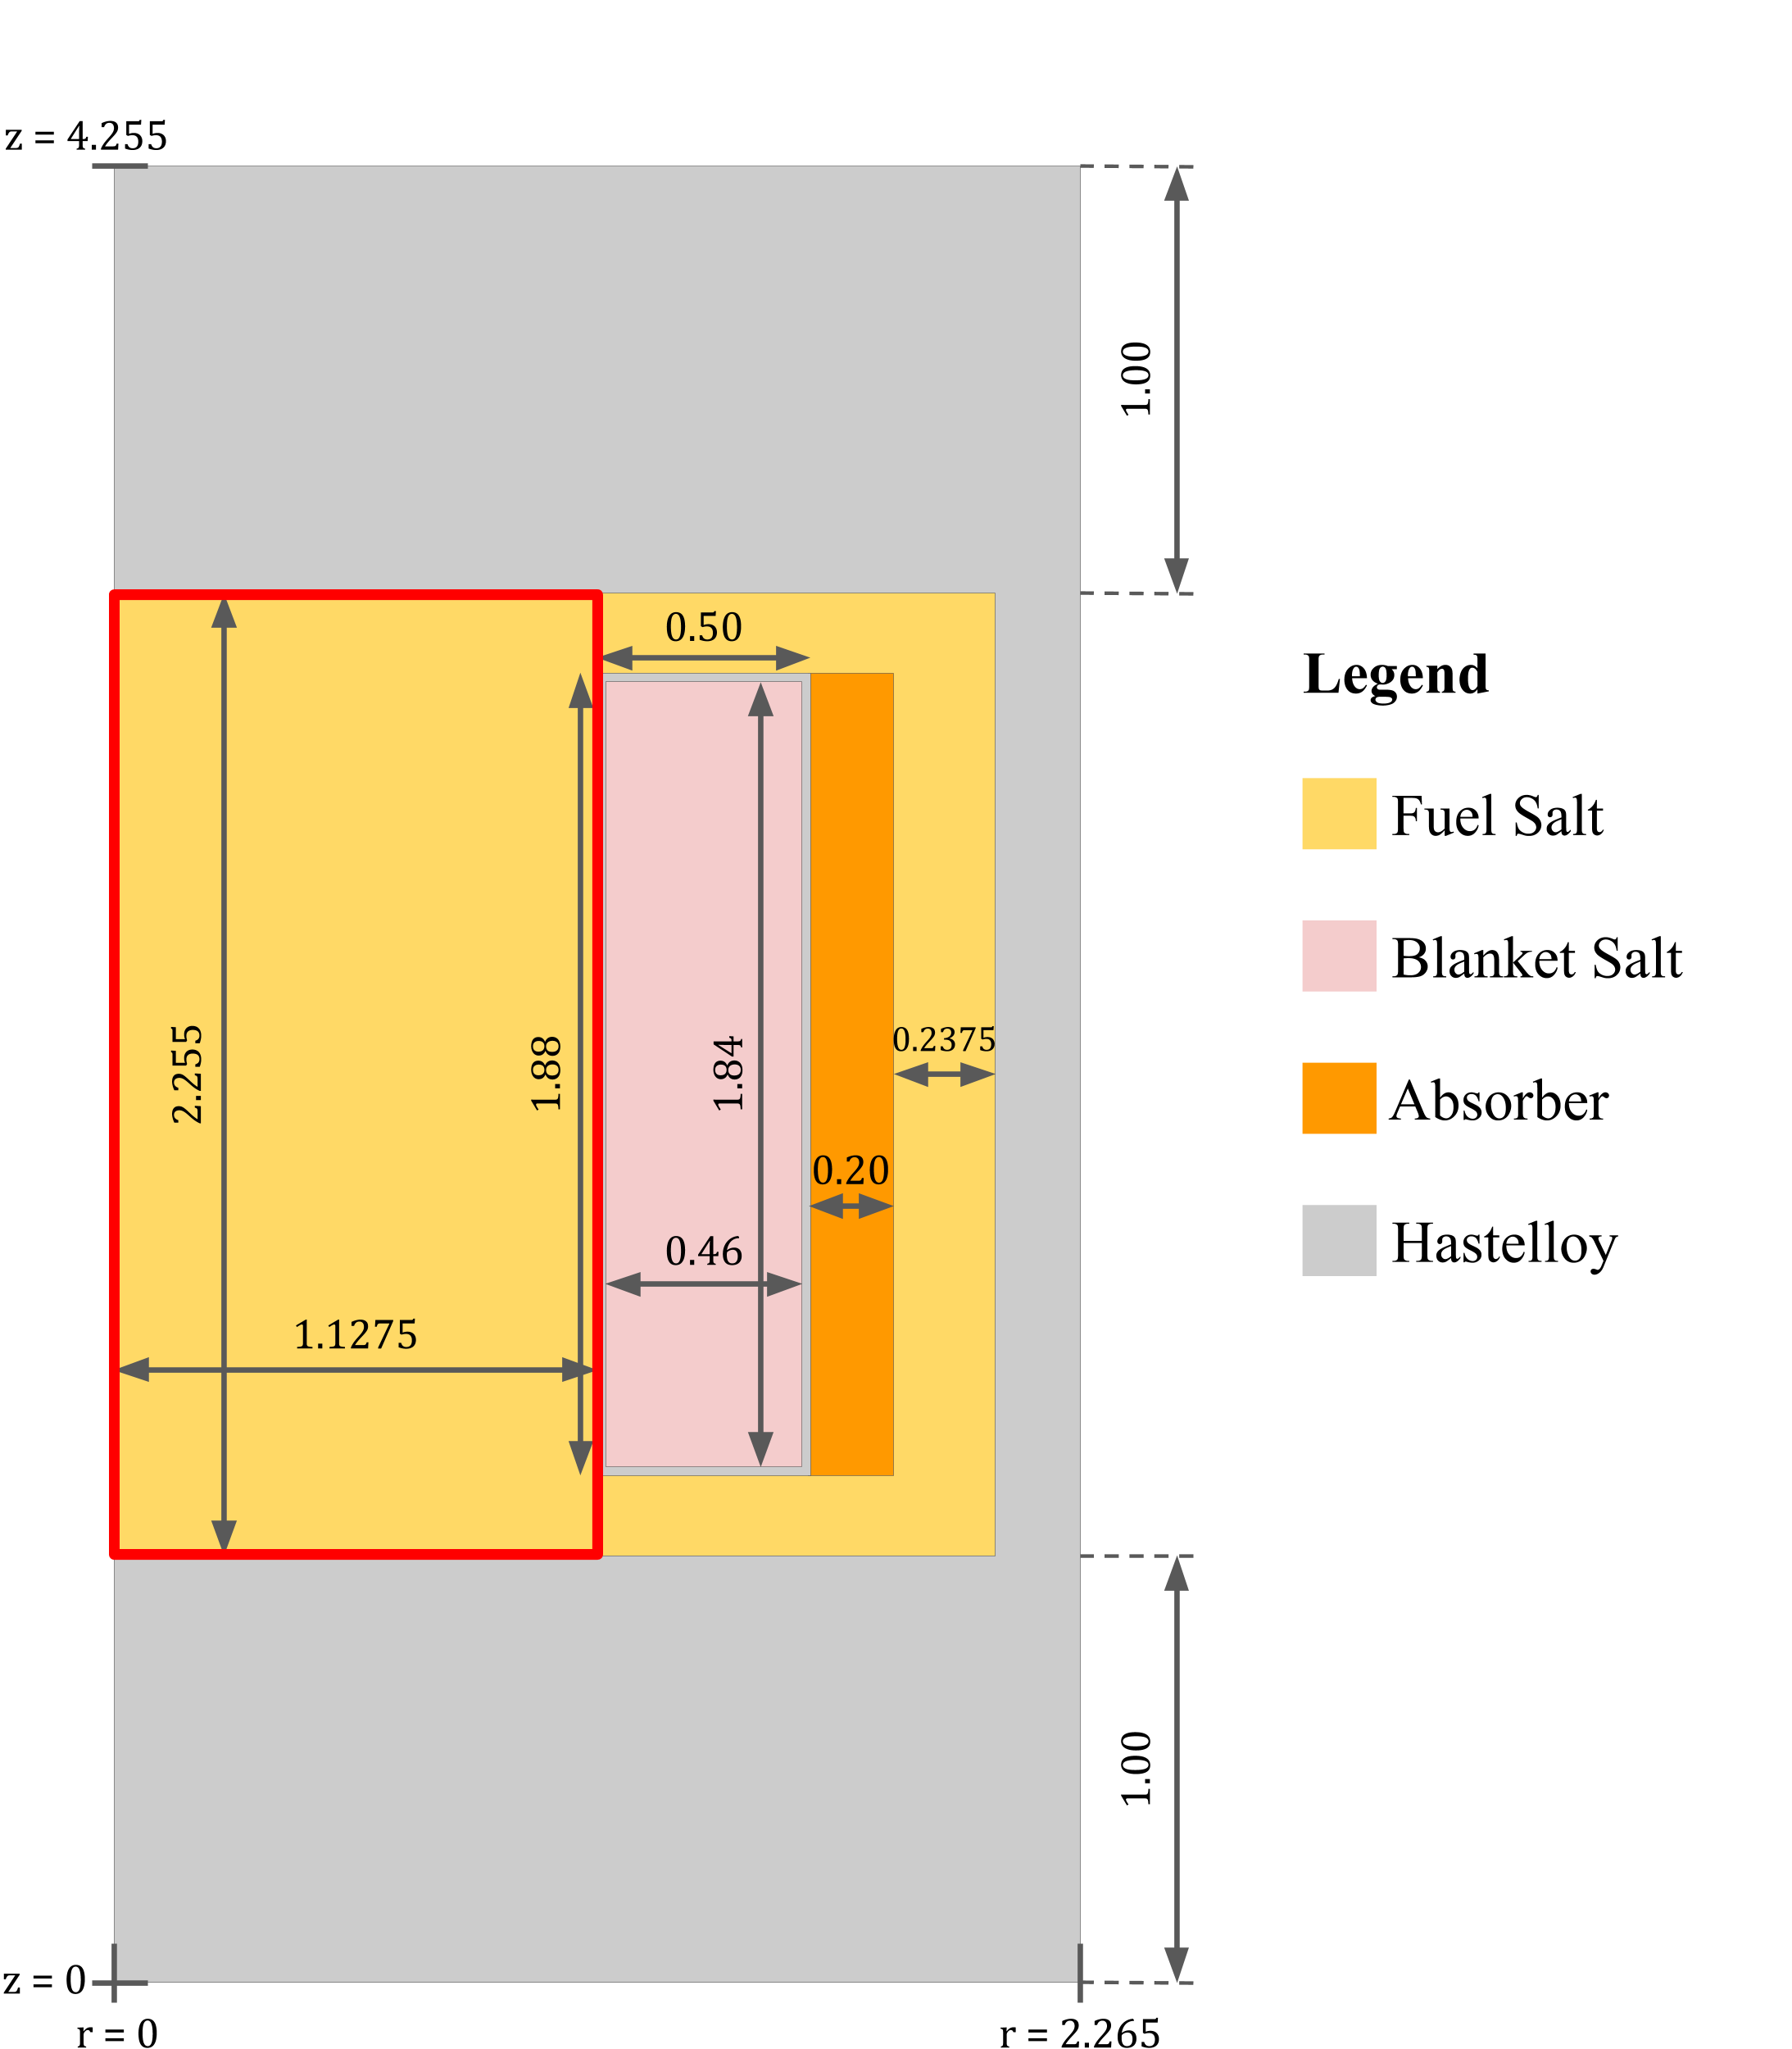
\includegraphics[width=.75\textwidth]{central-core-legend}
    \caption{2-D axisymmetric model of the MSFR. The red box indicates the
    central core region in the modeling approach in Moltres.}
    \label{fig:core}
\end{figure}

The central core region is of greatest interest to us during steady-state and
transient scenarios; the center of the reactor is naturally where most of the
fissions and heat generation occur.

\subsubsection{Neutronics Model}

Moltres performs neutron flux calculations in the central core region
using the standard formulations for the time-dependent multigroup
neutron diffusion equations and \gls{DNP} concentration equations as shown in
equations \ref{eq:neut} and \ref{eq:dnp}:
%
\begin{align}
    \frac{1}{v_g} \frac{\partial \phi_g}{\partial t} &= \nabla \cdot D_g
    \nabla \phi_g - \Sigma^r_g \phi_g +
    \sum^G_{g' \neq g} \Sigma^s_{g' \rightarrow g} \phi_{g'} + \chi^p_g
    \sum^G_{g'=1} (1-\beta) \nu \Sigma^f_{g'} \phi_{g'} + \chi^d_g \sum^I_i
    \lambda_i C_i, \label{eq:neut} \\
    \frac{\partial C_i}{\partial t} &= \beta_i \sum^G_{g'=1} \nu \Sigma^f_{g'}
    \phi_{g'} - \lambda_i C_i - \vec{u} \cdot \nabla C_i + \nabla \cdot
    K \nabla C_i, \label{eq:dnp} \\
    \intertext{where}
    v_g &= \text{average speed of neutrons in group $g$ [cm$\cdot$s$^{-1}$],} 
    \nonumber \\
    \phi_g &= \text{neutron flux in group $g$ [cm$^{-2}\cdot$s$^{-1}$],}
    \nonumber \\
    t &= \text{time [s],} \nonumber \\
    D_g &= \text{diffusion coefficient of neutrons in group $g$
    [cm$^2\cdot$s$^{-1}$],} \nonumber \\
    \Sigma^r_g &= \text{macroscopic cross section for removal of neutrons from
    group $g$ [cm$^{-1}$],} \nonumber \\
    \Sigma^s_{g' \rightarrow g} &= \text{macroscopic cross section of
    scattering from $g'$ to $g$ [cm$^{-1}$],} \nonumber \\
    \chi^p_g &= \text{prompt fission spectrum for neutrons in group $g$ [ - ],
    } \nonumber \\
    G &= \text{total number of discrete neutron groups [ - ],} \nonumber \\
    \nu &= \text{average number of neutrons produced per fission [ - ],}
    \nonumber \\
    \Sigma^f_{g} &= \text{macroscopic fission cross section for neutron in
    group $g$ [cm$^{-1}$],} \nonumber \\
    \chi^d_g &= \text{delayed fission spectrum for neutrons in group $g$
    [ - ],} \nonumber \\
    I &= \text{total number of delayed neutron precursor groups [ - ],}
    \nonumber \\
    \beta &= \text{total delayed neutron fraction [ - ],} \nonumber \\
    \beta_i &= \text{delayed neutron fraction of precursor group $i$ [ - ],}
    \nonumber \\
    \lambda_i &= \text{average decay constant of delayed neutron precursors in
    precursor group $i$ [s$^{-1}$],} \nonumber \\
    C_i &= \text{concentration of delayed neutron precursors in precursor
    group $i$ [cm$^{-3}$],} \nonumber \\
    K &= \text{turbulent diffusion coefficient of the delayed neutron
    precursors [cm$^2\cdot$s$^{-1}$].} \nonumber
\end{align}
%

While the limitations of the multigroup neutron diffusion method compared to
other deterministic and Monte Carlo methods, particularly for flux values near
boundaries, are well-documented, the diffusion model provides acceptable
accuracy at lower computational costs. Moreover, the central core region
contains no material interfaces except at its boundaries. Chapter
\ref{chap:nts} provides a comparison of the \gls{MSFR} multiplication factor
values and reactivity coefficients between Moltres and Serpent.

The \gls{DNP} concentration equation has additional advection and turbulent
diffusion terms to account for the movement of \glspl{DNP} in the primary
coolant loop. The turbulent diffusion $K$ is governed by the following
equation:
%
\begin{align}
    K &= \frac{\mu_t}{\rho Sc_t}
    \intertext{where}
    \mu_t &= \text{ eddy viscosity [Pa s],} \nonumber \\ 
    \rho &= \text{ density of the fuel salt [kg m$^{-3}$],} \nonumber \\
    Sc_t &= \text{ turbulent Schmidt number [ - ].} \nonumber
\end{align}
%
This work assumes $Sc_t = 0.85$ for a fair comparison with the Polimi and
TUDelft models \cite{fiorina_modelling_2014} which used the same value. It has
its roots in the Reynolds Analogy, which states that turbulent momentum and
heat transfer largely depend on the same eddies in turbulent flow
\cite{bartosiewicz_612_2019}. Therefore,
$Sc_t$ should be close to unity. $Sc_t = 0.85$ is also the default value for
most commercial \gls{CFD} software \cite{bartosiewicz_612_2019}.

\begin{figure}[htb!]
    \centering
    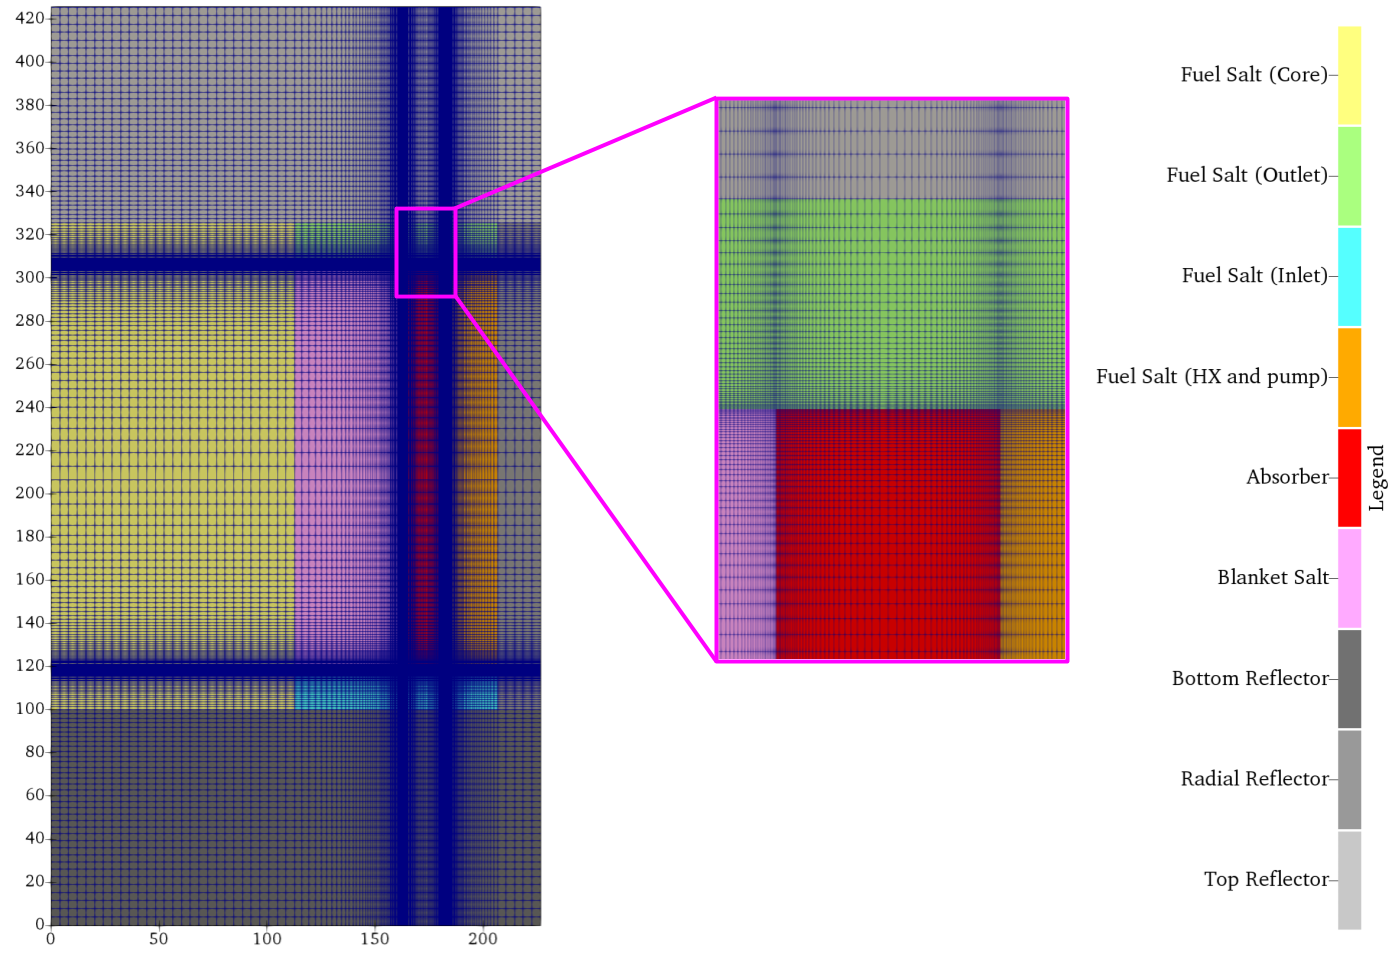
\includegraphics[width=\textwidth]{mesh2}
    \caption{Mesh adopted in Moltres and a close-up view of the mesh around
    the boron carbide absorber.}
    \label{fig:mesh}
\end{figure}

Moltres users can use an arbitrary number of neutron energy groups as
long as they provide Moltres with the appropriate group constant data. The
number of precursor groups is also variable, though usually predetermined by
the choice of nuclear data library in the group constant generation step.
Moltres automatically interpolates the group constant data for required
temperatures using one of the many predefined interpolation methods available
in \gls{MOOSE}. Once again, Moltres allows users to select their
interpolation method of choice.

This work uses six neutron energy groups according to the
energy boundaries in table \ref{table:bound}, and eight \gls{DNP} groups as
defined by the JEFF-3.1.2 library. The neutron flux
and \gls{DNP} concentration values were approximated by first-order Lagrange
and constant monomial shape functions respectively on the finite element mesh.
Figure \ref{fig:mesh} shows the mesh adopted for the \gls{MSFR} model.
This work assumes vacuum boundary conditions for all six neutron group fluxes
along the external boundaries of the geometry, and homogeneous Neumann
boundary conditions along the axial symmetry boundary. For the \gls{DNP}
concentrations, this work imposed homogeneous Neumann boundary conditions on
the walls, and inflow and outflow boundary conditions on the inlet and outlet
boundaries, respectively. The inlet \gls{DNP} concentration values were
imported from the outlet values of the 1-D outer loop pipe at the same
timestep. Table \ref{table:corebc} describes these boundary conditions
mathematically.

For the decay heat model, a previous study on the MSFR by Aufiero et al.
\cite{aufiero_extended_2013} showed that using three decay heat precursor
groups with appropriate half-lives in the form of exponential equations, can
accurately model decay heat in the MSFR for up to 300 seconds after shutdown
with a relative error of less than 2\%. Thus, this thesis implements the new
decay heat modeling capability with the following equation:
%
\begin{align}
	\frac{\partial \omega_j}{\partial t} &= f_j \sum^G_{g=1} \epsilon_{g}
	\Sigma^f_{g} \phi_{g} - \lambda_j \omega_j - \vec{u} \cdot \nabla
	\omega_j + \nabla \cdot K \nabla \omega_j, \label{eq:decayheat} \\
	\intertext{where}
    \omega_j &= \text{total decay heat power density from decay heat
    precursors in group $j$ [W$\cdot$cm$^{-3}$],} \nonumber \\
	f_j &= \text{fraction of total power attributable to decay heat group
	$j$ [ - ],} \nonumber \\
	\epsilon_g &= \text{average fission energy per fission initiated by a
	neutron in group $g$ [W],} \nonumber \\
	\lambda_j &= \text{average decay constant of decay heat precursors in
	group $j$ [s$^{-1}$].} \nonumber
\end{align}

Like the neutron energy and \gls{DNP} groups, Moltres can accommodate an
arbitrary number of decay heat groups. The current work uses the same decay
heat fractions and decay constants, shown in Table \ref{eq:decayheat}, used in
the Polimi and TUDelft models for three decay heat groups.

\begin{table}[htb!]
	\centering
	\caption{Decay heat group parameters \cite{fiorina_modelling_2014}.}
	\begin{tabular}{S S S}
		\toprule
		{Decay heat group $j$} & {$\lambda_j$ [s$^{-1}$]} & {$f_j$} \\
		\midrule
		1 & 0.1974 & 0.0117 \\
		2 & 0.0168 & 0.0129 \\
		3 & 0.000358 & 0.0186 \\
		\bottomrule
	\end{tabular}
	\label{table:decayheat}
\end{table}

\subsubsection{Thermal-Hydraulics Model}

This work models fluid dynamics using the \gls{INS} capabilities from the
MOOSE Navier-Stokes module \cite{peterson_overview_2017}. The standard
\gls{INS} equations are:
%
\begin{align}
    \text{Momentum eq.:} && \rho \frac{\partial \vec{u}}{\partial t} &=
    -\rho (\vec{u}
    \cdot \nabla) \vec{u} + \nabla \cdot [-p \vec{I} + \mu [
    \nabla \vec{u} + (\nabla \vec{u})^T]] + \vec{f} &&
    \label{eq:momemtum} \\
    \text{Divergence-free:} && \nabla \cdot \vec{u} &= 0 &&
    \label{eq:divergence}
    \intertext{where}
    && p &= \text{ pressure [Pa],} && \nonumber \\
    && \mu &= \text{ dynamic viscosity [Pa$\cdot$s],} && \nonumber \\
    && \vec{f} &= \text{ body force per unit volume [N$\cdot$m$^{-3}$].} &&
    \nonumber
\end{align}

In addition to the intrinsic molecular viscosity in the \gls{INS} equations,
this thesis includes an eddy viscosity term, $\mu_t$, to approximate
turbulent flow effects. The current implementation of the Navier-Stokes module
does not have a turbulence model. The options for turbulence modeling in
\gls{CFD} include direct numerical simulations (DNS) and large eddy
simulations (LES) for higher fidelity flow simulations, \gls{RANS} methods for
balanced compromises between accuracy and computational speed, and lumped
parameter and sub-channel methods for even faster performance with greater
accuracy costs \cite{moorthi_review_2018}. The Polimi and TUDelft models used
\gls{RANS} methods to model salt flow \cite{fiorina_modelling_2014}. This work
uses a zeroth-order approximation of $\mu_t$ based on the calculated $\mu_t$
values reported in the Polimi and TUDelft models. The models predicted spatial
$\mu_t$ values ranging from 0 to 110 Pa$\cdot$s, with most values
falling within the 30 to 50 Pa$\cdot$s range. Thus, the present work uses
the approximated value $\mu_t=$ 40 Pa$\cdot$s. Despite the simplicity of this
approximation, the resulting flow profile is similar to the flow profile in
the Polimi and TUDelft models at steady-state.

The energy balance equation for temperature used in this Moltres model is:
%
\begin{align}
    \rho c_{p} \frac{\partial T}{\partial t} &= - \rho c_p \vec{u}
    \cdot \nabla T + \nabla \cdot [(k + k_t) \nabla T] + Q_s
    \label{eq:temp} \\
    k_t &= \frac{\mu_t}{\rho Pr_t} \\
    Q_s &= \Big( 1 - \sum^J_{j=1} f_j \Big) \sum^G_{g=1} \epsilon_g \Sigma_g^f
    \phi_g + \sum^J_{j=1} \omega_j, \label{eq:source}
    \intertext{where}
    c_p &= \text{specific heat capacity of molten salt
    [J$\cdot$kg$^{-1}\cdot$K$^{-1}$],} \nonumber \\
    T &= \text{temperature of molten salt [K]} \nonumber \\
    \vec{u} &= \text{velocity of molten salt [m$\cdot$s$^{-1}$],}
    \nonumber \\
    k &= \text{thermal conductivity of molten salt
    [W$\cdot$m$^{-1}\cdot$K$^{-1}$],} \nonumber \\
    J &= \text{total number of decay heat groups [ - ].} \nonumber
\end{align}
%
The diffusion term includes turbulent heat
diffusivity based on the eddy viscosity $\mu_t$ and the turbulent Prandtl
number $Pr_t$. $Pr_t$ is also 0.85 due to the same reasoning provided for
$Sc_t$. The first term in the heat source $Q_s$ equation represents prompt
fission heat, and the second term represents decay heat from the $J$ decay
heat groups.

With this model, the results were expected to show good qualitative agreement
with the Polimi and TUDelft models, including the large recirculation region
near the blanket tank walls and the resulting high temperatures in that
region. The results in Chapter \ref{chap:ss} show minor discrepancies in
regions where the viscosity values were under- or over-predicted.

\subsubsection{Boundary Conditions}

Table \ref{table:corebc} summarizes the boundary conditions for all variables
on all of the relevant boundaries. Figure \ref{fig:msfrbc} shows the locations
of the various boundaries listed in the table. The CoupledOutflow boundary
condition for $C_i$ and $\omega_j$ is a new feature in Moltres that allows
users to couple these variables to the outlet velocity components (e.g. $u_x$,
$u_y$). Without this boundary condition, users could only use uniform or fixed
function-based velocity profiles in conjunction with the precursor looping
capability.

\begin{table}[htbp!]
    \small
	\caption{Boundary conditions in the main reactor geometry (Figure
	\ref{fig:msfrbc}).}
	\centering
	\begin{tabular}{ l l c}
		\toprule
		Variable & Boundary & Boundary Condition \\
		\midrule
		\multirow{4}{*}{Neutron flux $\phi_g$} & Top & $\frac{d \phi_g}{dx}
		\big|_{\text{inflow}} = 0$ \\[.5ex]
        & Outer & $\frac{d \phi_g}{dx} \big|_{\text{inflow}} = 0$ \\[.5ex]
        & Bottom & $\frac{d \phi_g}{dx} \big|_{\text{inflow}} = 0$ \\[.5ex]
        & Axial & $\frac{d \phi_g}{dx} = 0$ \\[.5ex]
        \midrule
        \multirow{6}{*}{Delayed neutron precursor concentration $C_i$} &
        Top (Core) & $\frac{d C_i}{dx} = 0$ \\[.5ex]
        & Bottom (Core) & $\frac{d C_i}{dx} = 0$ \\[.5ex]
        & Outer (Core) & $\frac{d C_i}{dx} = 0$ \\[.5ex]
        & Axial (Core) & $\frac{d C_i}{dx} = 0$ \\[.5ex]
        & Inlet (Core) & $C_i = c$ \\
        & Outlet (Core) & $u_x \cdot C_i = 0$ \\
        \midrule
        \multirow{6}{*}{Decay heat power density $\omega_j$} &
        Top (Core) & $\frac{d \omega_j}{dx} = 0$ \\[.5ex]
        & Bottom (Core) & $\frac{d \omega_j}{dx} = 0$ \\[.5ex]
        & Outer (Core) & $\frac{d \omega_j}{dx} = 0$ \\[.5ex]
        & Axial (Core) & $\frac{d \omega_j}{dx} = 0$ \\[.5ex]
        & Inlet (Core) & $\omega_j = c$ \\
        & Outlet (Core) & $u_x \cdot \omega_j = 0$ \\
        \midrule
        \multirow{6}{*}{Radial velocity $u_x$} & Top (Core) & $u_x = 0$ \\
        & Bottom (Core) & $u_x = 0$ \\
        & Outer (Core) & $u_x = 0$ \\
        & Axial (Core) & $u_x = 0$ \\
        & Inlet (Core) & $u_x = c$ \\
        & Outlet (Core) & $\frac{d u_x}{dx} = 0$ \\[.5ex]
        \midrule
        \multirow{6}{*}{Axial velocity $u_y$} & Top (Core) & $u_y = 0$ \\
        & Bottom (Core) & $u_y = 0$ \\
        & Outer (Core) & $u_y = 0$ \\
        & Axial (Core) & $\frac{d u_y}{dx} = 0$ \\[.5ex]
        & Inlet (Core) & $u_y = 0$ \\
        & Outlet (Core) & $\frac{d u_y}{dx} = 0$ \\[.5ex]
        \midrule
        \multirow{6}{*}{Temperature $T$} & Top (Core) &
        $\frac{d T}{dx} = 0$ \\[.5ex]
        & Bottom (Core) & $\frac{d T}{dx} = 0$ \\[.5ex]
        & Outer (Core) & $\frac{d T}{dx} = 0$ \\[.5ex]
        & Axial (Core) & $\frac{d T}{dx} = 0$ \\[.5ex]
        & Inlet (Core) & $T = c$ \\
        & Outlet (Core) & $\frac{d T}{dx} = 0$ \\[.5ex]
		\bottomrule
	\end{tabular}
	\label{table:corebc}
\end{table}

\clearpage

\begin{figure}[htb!]
    \centering
    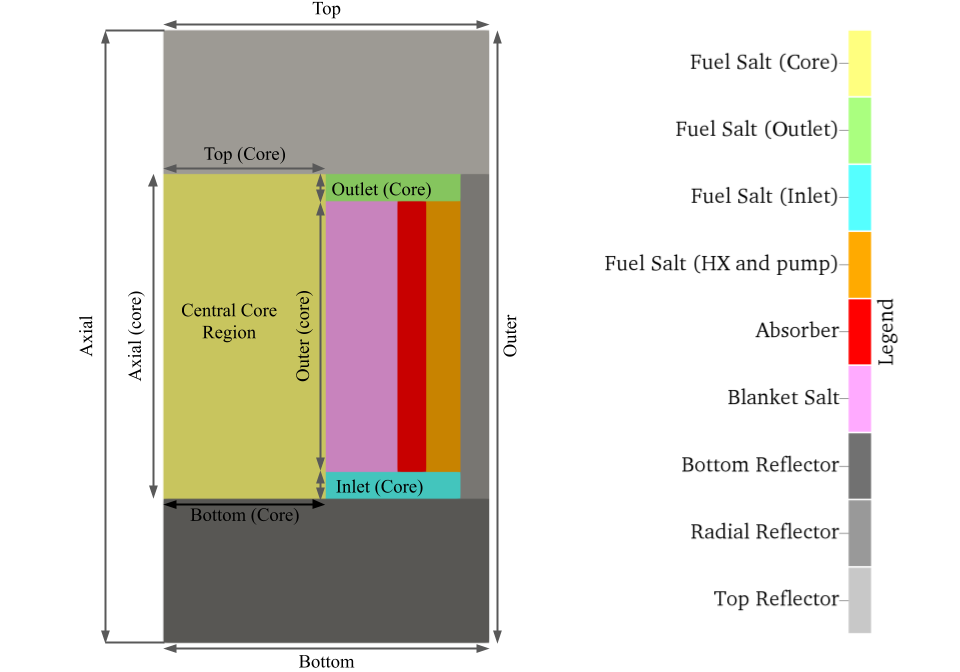
\includegraphics[width=.8\textwidth]{msfrbc}
    \caption{The boundaries in the \gls{MSFR} geometry that are relevant for
    the boundary conditions mentioned in Table \ref{table:corebc}.}
    \label{fig:msfrbc}
\end{figure}

\subsection{Outer Loop Region}

Moltres also accounts for the decay of
\glspl{DNP} outside the central core region by simulating its flow in a
separate 1-D pipe geometry. This outer loop pipe calculation is implicitly
coupled to the active core simulation through Picard iterations in MOOSE's
MultiApp functionality and inlet/outlet boundary values. For this work with
the \gls{MSFR} model, the pipe length is 2.255 m with salt flowing at 1.1275 m
s$^{-1}$ for an out-of-core residence time of 2 s. The present author derived
these parameters from the reference specifications of 4s cycle
time and 50\% out-of-core salt fraction (Table \ref{table:msfr}).

\subsubsection{Neutronics Model}

The outer loop region is largely subcritical because most of it is adjacent to
the boron carbide absorber as shown in Figure \ref{fig:core}. Therefore, the
only significant neutronics-related phenomena are the drift and decay of
\glspl{DNP}. The governing equation for the \glspl{DNP} is:
%
\begin{align}
    \frac{\partial C_i}{\partial t} &= - \lambda_i C_i - u
    \frac{\partial C_i}{\partial x}.
    \label{eq:dnploop}
\end{align}
%
Equation \ref{eq:dnploop} is derived from equation \ref{eq:dnp} by removing
the fission \gls{DNP} source term, and the conversion of the advection and
diffusion terms to their 1-D forms. The decay constants and diffusion
coefficient are the same values used in the central core region.

\subsubsection{Thermal-Hydraulics Model}

A constant velocity of 1.1275 m s$^{-1}$ is applied in the outer loop region
to maintain the nominal 2s out-of-core residence time. The governing equation
for temperature, derived from equation \ref{eq:temp}, is:
%
\begin{align}
    \rho c_{p} \frac{\partial T}{\partial t} &= - \rho c_p u
    \frac{\partial T}{\partial x} - Q_{hx} \label{eq:temploop} \\
    Q_{hx} &= \alpha (T - T_i) \delta (x_0) \label{eq:hx} \\
    \intertext{where}
    Q_{hx} &= \text{heat removal rate through the heat exchanger [W],} 
    \nonumber \\
    \alpha &= \text{heat transfer coefficient [W$\cdot$K$^{-1}$],} \nonumber
    \\
    T_i &= \text{temperature of the intermediate salt [K],} \nonumber \\
    x_0 &= \text{position of the point heat exchanger [m].} \nonumber
\end{align}

In the outer loop region, the fission heat source term is replaced with a heat
exchanger sink term $Q_{hx}$
which depends on the temperature difference between the fuel salt $T$ and the
intermediate loop salt $T_i$. For simplicity, this work assumes a constant
temperature of 823 K in the intermediate loop. The heat transfer coefficient
was determined by assuming that the fuel outlet temperature is 1023 K and
calculating the heat removal rate to induce a 100 K drop at the given
volumetric flow rate and heat capacity of the fuel salt. The resulting value
for $\alpha$ is 370.668 W$\cdot$K$^{-1}$. This work opted to
ignore the diffusion term due to the discontinuity of the temperature
distribution across the point heat exchanger. 

\subsubsection{Boundary Conditions}

Table \ref{table:loopbc} summarizes the boundary conditions for all variables
on the inlet and outlet of the 1-D outer loop region. The inlet boundary
conditions are all Dirichlet boundary conditions. The inlet boundary values
are set by the outflow from the central core region that this inlet is
connected to in the actual reactor geometry. The outlet boundary conditions
are all outflow boundary conditions as shown in Table \ref{table:loopbc}.

\begin{table}[htbp!]
    \small
	\caption{Boundary conditions in the 1-D outer loop geometry. $u$
	represents the 1-D velocity in this region.}
	\centering
	\begin{tabular}{ l l c}
		\toprule
		Variable & Boundary & Boundary Condition \\
        \midrule
        \multirow{2}{*}{Delayed neutron precursor concentration $C_i$} &
        Inlet (Core) & $C_i = c$ \\
        & Outlet (Core) & $u \cdot C_i = 0$ \\
        \midrule
        \multirow{2}{*}{Decay heat power density $\omega_j$} &
        Inlet (Core) & $\omega_j = c$ \\
        & Outlet (Core) & $u \cdot \omega_j = 0$ \\
        \midrule
        \multirow{2}{*}{Temperature $T$} &
        Inlet (Core) & $T = c$ \\
        & Outlet (Core) & $u \cdot T = 0$ \\
		\bottomrule
	\end{tabular}
	\label{table:loopbc}
\end{table}

\subsection{Central Core and Outer Loop Coupling}

This subsection details the delayed neutron and decay heat precursors, and
temperature coupling between the central core and outer loop regions. 

%Starting with the central core region, for the neutron group fluxes, we
%imposed vacuum boundary conditions on the
%outermost boundaries of the geometry in Figure \ref{fig:core} excluding the
%axial boundary. The \gls{DNP} variables have homogeneous Neumann boundary
%conditions along the axis and the walls in the central core region, and inflow
%and outflow boundary conditions on the inlet and outlet boundaries,
%respectively. The temperature variable shares the same type of boundary
%conditions as the \gls{DNP} variables.

This work uses a parabolic flow profile on the inlet Dirichlet boundary
condition. The equation for $u_x$ at the inlet is:
%
\begin{align}
    u_x &= -\xi \Big[\frac{y}{H} - \Big(\frac{y}{H}\Big)^2 
    \Big] \\
    \intertext{where}
    \xi &= \text{normalizing constant [m$\cdot$s$^{-1}$],} \nonumber \\
    y &= \text{height along the inlet [m],} \nonumber \\
    H &= \text{total height of the inlet $= 0.1875$ m.} \nonumber
\end{align}
%
$\xi$ is a normalizing constant that depends on the total volumetric flow
rate, $\dot{V}$. Solving the following set of equations in $v$ and $\dot{V}$:
%
\begin{align}
    v &= \xi [\frac{y}{H} - \frac{y^2}{H^2}] \\
    \dot{V} &= \int^h_0 \int^{2 \pi}_0 v r d\theta dy \\
    \intertext{where}
    r &= \text{radius [m],} \nonumber \\
    \theta &= \text{azimuthal angle [rad],} \nonumber
\end{align}
%
gives $\xi = 20.3401$ m$\cdot$s$^{-1}$ for $\dot{V} = 4.5$ m$^3\cdot$s$^{-1}$. 

At every timestep, Moltres also calculates weighted averages of the
temperature and the precursors at the outlet. These values are weighted by the
outflow velocity values at the outlet according to the following equation:
%
\begin{align}
    \overline{\psi} &= \frac{\int_\mathcal{C} \psi(y) u(y) dy}{
    \int_\mathcal{C} u(y) dy} \\
    \intertext{where}
    \psi &= \text{variable to be weighted [ - ]} \nonumber \\
    \mathcal{C} &= \text{outlet boundary area [ - ]} \nonumber \\
    u &= \text{outflow velocity perpendicular to the outlet boundary
    [m$\cdot$s$^{-1}$].} \nonumber
\end{align}

Moltres transfers this outflow value from the central core region to the 1-D
outer loop region, to be used as the boundary value for the inhomogeneous
Dirichlet boundary
condition at the inlet. Likewise, the outflow value from the outer
loop region is used for the inflow value in the central core region. No
averaging is required for this step as the outer loop region is a 1-D system.
We assume that the inflow temperature and \gls{DNP} are uniform at the inlet.
The Picard iterations within every timestep ensure that the two systems are
implicitly coupled even though they're solved separately.
